Se pide hacer un filtrado en frecuencia del archivo \texttt{nspeech.mat}, el cual presenta un tono molesto.

En primer lugar se obtiene la DFT de dicha señal y se grafica su magnitud en frecuencia, encontrando un peak en los 1685 Hz, localizando así el tono molesto. El gráfico obtenido se muestra en la figura \ref{fig:p3_1cf}.

\begin{figure}[H]
    \centering
    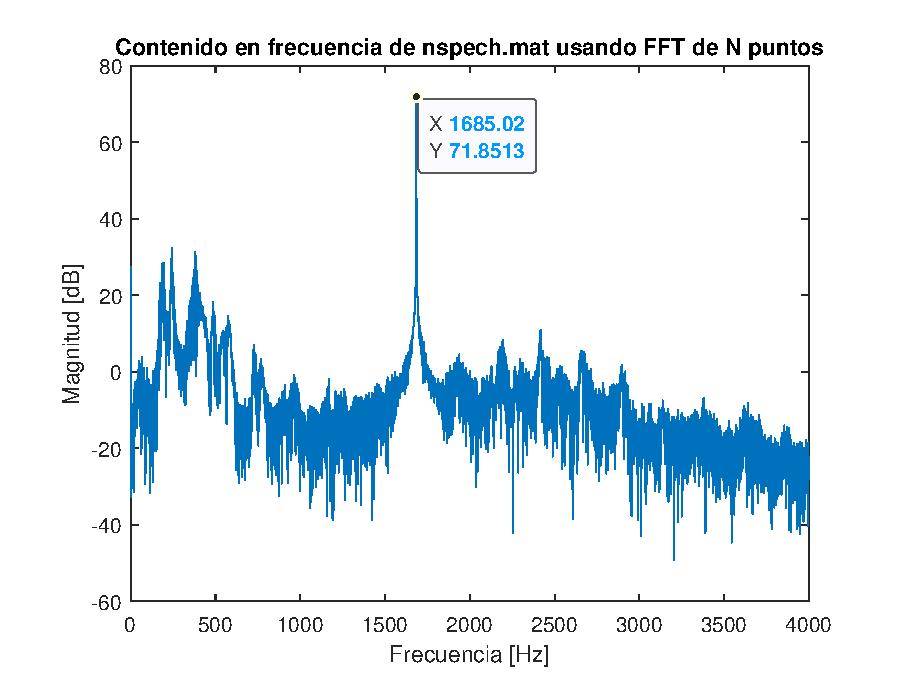
\includegraphics[width = .8\linewidth]{Figuras/p3_1cf.eps}
    \caption{Contenido en frecuencia (magnitud) de señal \texttt{nspeech.mat}.}
    \label{fig:p3_1cf}
\end{figure}

Posteriormente se diseña un filtro de 2 ceros conjugados, de respuesta en frecuencia:
$$ H(\omega) = 1-2\cos{(\theta)e^{-j\omega}+e^{-2j\omega}}$$
Donde se ubican los ceros en el ángulo correspondiente a la frecuencia normalizada del tono molesto, es decir 
$$ \theta = 2\pi \dfrac{f_0}{f_s} =2\pi \dfrac{1685}{8000} = 1.322~ \dfrac{\text{rad}}{\text{muestra}}$$
Con el objetivo de penalizar dicha frecuencia. La magnitud de la respuesta en frecuencia del filtro diseñado se muestra en la figura \ref{fig:p3_2rfH}. Se aprecia la penalización correspondiente en la frecuencia del tono molesto. 

\begin{figure}[H]
    \centering
    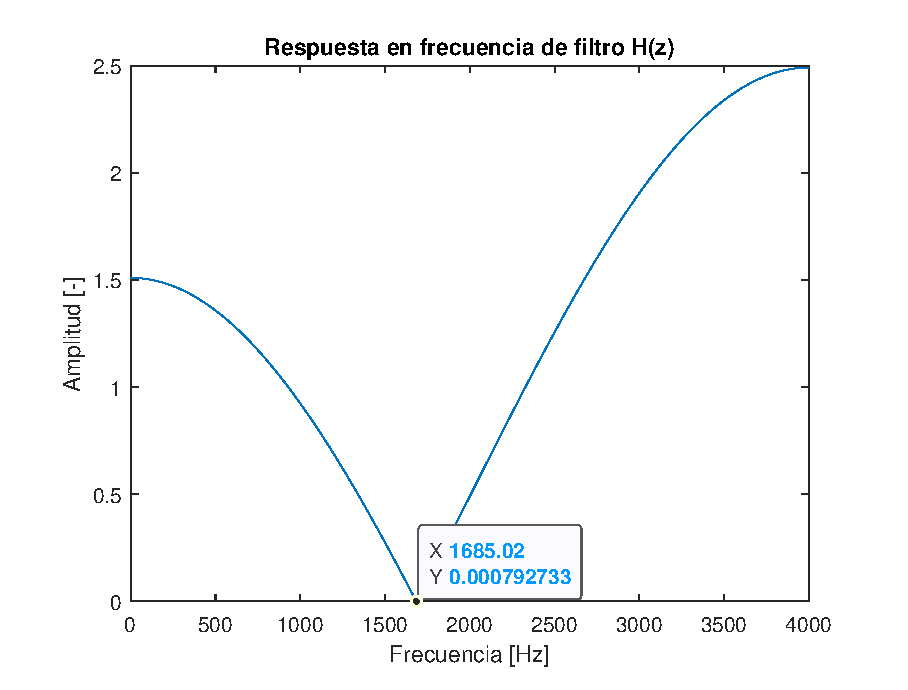
\includegraphics[width = .8\linewidth]{Figuras/p3_2rfH.eps}
    \caption{Respuesta en frecuencia (magnitud) de filtro de 2 ceros complejos conjugados diseñado.}
    \label{fig:p3_2rfH}
\end{figure}

Ya con el filtro diseñado, se realiza el filtrado en frecuencia haciendo un producto punto a punto de las respuestas en frecuencia del contenido en frecuencia de la señal \texttt{nspeech.mat} y la respuesta en frecuencia de $H$, teniendo cuidado con que la discretización en frecuencia de la expresión de $H(\omega)$ corresponda a la frecuencia de los bines de la DFT de la señal original.

La magnitud del contenido en frecuencia de la señal filtrada se muestra en la figura \ref{fig:p3_3cffilt}. En comparación con la figura \ref{fig:p3_1cf} se aprecia una gran atenuación, más no eliminación del tono molesto. Lo anterior se le atribuye a temas numéricos.

\begin{figure}[H]
    \centering
    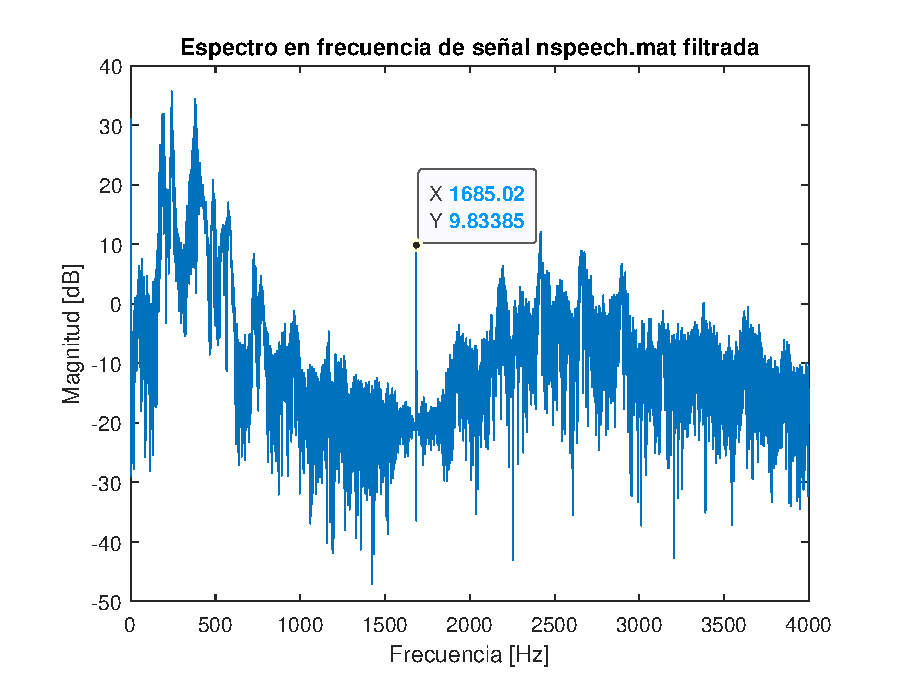
\includegraphics[width = .8\linewidth]{Figuras/p3_3cffilt.eps}
    \caption{Contenido en frecuencia (magnitud) de señal \texttt{nspeech.mat} filtrada.}
    \label{fig:p3_3cffilt}
\end{figure}

Finalmente se aplica la DFT inversa a la señal filtrada en el dominio de la frecuencia para obtener su representación en el dominio del tiempo. Los gráficos de la señal pre y post filtrado se muestran en la figura \ref{fig:p3_4tiempo}. Visualmente aprecian buenos resultados producto al filtrado. Con respecto al número de puntos para recuperar la señal completa, corresponde al número de puntos de la señal \texttt{nspeech.mat}.

\begin{figure}[H]
    \centering
    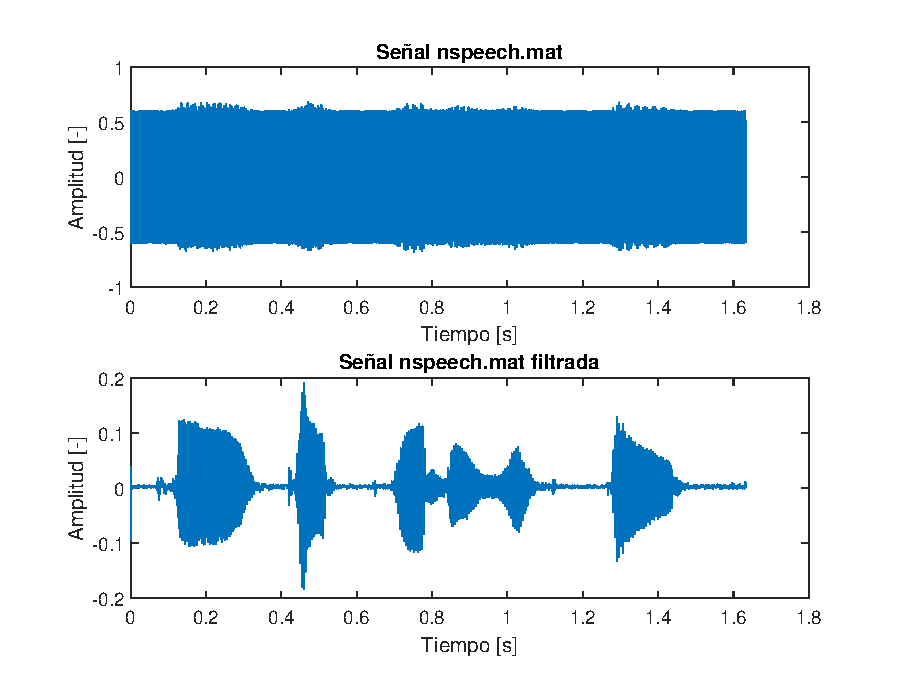
\includegraphics[width = .8\linewidth]{Figuras/p3_4tiempo.eps}
    \caption{Representación de señal pre y post filtrado en el dominio temporal.}
    \label{fig:p3_4tiempo}
\end{figure}

Con respecto a la percepción auditiva, se aprecia una gran disminución del tono molesto, sin embargo, sigue sonando levemente. Se adjuntan archivos de audio \texttt{nspeech\_filtered.wav} y \texttt{nspeech\_unfiltered.wav} a la entrega.